\chapter{Empirischer Teil} % Main chapter title

\label{K5} % Change X to a consecutive number; for referencing this chapter elsewhere, use \ref{Chapter4}

%------------------------------------------------------

Der empirische Teil der vorliegenden Arbeit umfasst eine allgemeine Umfrage zur Nutzung von Skype (s. Kap.\,\ref{K6:sec:UmfrageAllg} und Anhang \ref{App:F1}, S.\,\pageref{App:F1}) sowie eine Fallstudie, mit der die Wahrnehmung der Chat-Kommunikation unter Einsatz des Skype Translators\is{Skype!Skype Translator} untersucht werden soll. Auch wenn die Online-Umfrage nicht den Anspruch erhebt, umfassend und repräsentativ zu sein, sollen die Ergebnisse dazu dienen, die Wahrnehmung und die Nutzung von Skype -- und im Speziellen des Skype Translators -- besser einordnen zu können. An dieser Stelle sei bereits darauf hingewiesen, dass der gesamte empirische Teil pilotiert wurde. Um inhaltliche, organisatorische, logische und orthographische Fehler zu erkennen und zu beheben, wurden die Fragebögen vorweg an nicht beteiligte Personen weitergeleitet. Auch die Kommunikationssituation\is{Kommunikation!-ssituation} über Skype wurde -- um nicht zuletzt die reibungslose Integration des Eye-Trackers in den Versuchsaufbau zu gewährleisten -- vorab mit unbeteiligten Personen überprüft. Auf Grundlage der während der Pilotierung\is{Pilotierung} gewonnen Erkenntnisse wurde für die Teilnehmer{\textperiodcentered}innen ein Einweisungstext samt rechtlicher Hinweise ausgearbeitet, der im Anhang ersichtlich ist (s. Anhang \ref{App2:EinweisungEva}, S.\,\pageref{App2:EinweisungEva}). Alle weiteren Details den Aufbau und die Durchführung betreffend werden in den entsprechenden Unterkapiteln dargelegt. Zitate aus den Angaben der Proband{\textperiodcentered}innen werden im Folgenden als Original mit Orthographie- und Interpunktionsfehlern dargestellt.

%------------------------------------------------------------------------

\section{Begrifflicher Hinweis}
\label{K5:sec:begrifflicher-hinweis}

%------------------------------------------------------------------------

Um Missverständnisse bei der Darstellung der nachfolgenden Studie zu vermeiden, sei hier noch kurz die verwendete Terminologie aufgeführt:

\begin{description}\sloppy
    \item[Chatbeitrag:] Jegliche textuelle Äußerung von einer der beiden am Gespräch beteiligten Personen, die über die Eingabemaske von Skype in den Chat eingebracht und versendet wurde, sodass sie für die beiden Gesprächspartner{\textperiodcentered}innen sichtbar wurde. Üblicherweise löst ein Chatbeitrag unter Verwendung des Skype Translators\is{Skype!Skype Translator} automatisch die maschinelle Übersetzung in die jeweils andere Sprache aus.\is{Chat!-beitrag}
    
    \item[eingehende Nachrichten:] Unter eingehenden Nachrichten sind alle Nachrichten zu verstehen, die als neue Information an die Proband{\textperiodcentered}innen im Rahmen der Kommunikationssituation\is{Kommunikation!-ssituation} herangetragen werden. Die MÜ-Ausgabe der von den Proband{\textperiodcentered}innen selbst verfassten Nachrichten zählt nicht zu eingehenden Nachrichten.
    
    \item[ausgehende Nachrichten:] Ausgehende Nachrichten wiederum sind die Chatbeiträge\is{Chat!-beitrag}, die von den Proband{\textperiodcentered}innen selbst verfasst wurden. Hierzu zählt auch die MÜ-Ausgabe der von den Proband{\textperiodcentered}innen selbst verfassten Nachrichten.
\end{description}

%------------------------------------------------------------------------

\section{Methodik}
\label{K5:sec:Methodik}

%------------------------------------------------------------------------


%------------------------------------------------------------------------

\subsection{Online-Befragung}
\label{K5:subsec:Online-Befragung}

%------------------------------------------------------------------------

Das Erhebungsverfahren der wissenschaftlichen Umfrage\is{Umfrage|(} ist ein vielseitiges Feld. Fragebögen\is{Fragebogen} werden heutzutage nicht nur in gedruckter Form verteilt, sondern können auch als Online-Version den zu Befragenden zugänglich gemacht werden. Eine Telefonumfrage\is{Umfrage!Telefon-} sowie der Versand von Fragebögen\is{Fragebogen|(} per Post kann dabei ebenfalls zu dieser Kategorie gezählt werden.

Für die Wahl des Erhebungsverfahrens sind mehrere Faktoren entscheidend. Zunächst einmal steht die Aufwand-Nutzen-Abwägung im Vordergrund. Der Fragebogen bzw. die Umfrage gelten als zeit- und ressourcensparend sowie einfach durchzuführen \citep[59]{albert_empirisches_2014}. Weiterhin ist die Grundgesamtheit der Zielgruppe ebenso zu beachten wie die generelle Erreichbarkeit (sprich: der Zugang zu) dieser Gruppe. Auch die Reaktivität sollte vorab in die Konzeption miteinbezogen werden, da nicht jede befragte Person gleichermaßen gerne Online-Fragebögen, analoge oder Telefonumfragen beantwortet. Bei der persönlichen Befragung bzw. der Papierumfrage kann es zum sog. \glqq Interviewer-Effekt\grqq\,(ebd., auch \emph{observer's paradox}) kommen, bei der die befragte Person von der Gesamtsituation beeinflusst wird und dies zu einer Verzerrung der Antworten führt. Dieser Effekt tritt bei Online-Umfragen selten bis überhaupt nicht auf. Zugleich sollte bei der Konzeption aber bedacht werden, dass Fragebögen lediglich \glqq die subjektiven Einschätzungen der befragten Person zu den Themen der Befragung (...) erfassen\grqq{} \citep[164]{aeppli_empirisches_2016} und somit einer möglichen Verzerrung der Antworten durch die gegenwärtige Gefühlslage der befragten Personen unterliegen.

\begin{sloppypar}
Ein Nachteil der Online-Befragung\is{Umfrage!online} ist die Kontrollierbarkeit. Das Ausfüllen findet ohne die Möglichkeit für die befragte Person statt, bei Unklarheiten Rückfragen an den Wissenschaftler zu stellen. Auch kann es zu Missverständnissen bei der Formulierung der einzelnen Fragen kommen, sodass die Ergebnisse durch eine unzureichende Konzeption von vornherein verzerrt sind. Dieses Problem kann durch eine tiefgreifende, ausführliche Pilotierung\is{Umfrage!Pilotierung}, also einem Testlauf bzw. Pretest\is{Umfrage!Pretest}, umfassend eingegrenzt werden \citep[61]{aeppli_empirisches_2016}. Nicht zuletzt liegt die Rücklaufquote von Online-Befragungen häufig unter der der anderen Umfragearten \citep[165]{aeppli_empirisches_2016}. Ferner kann bei der Bereitstellung von Online-Umfragen nie vollständig gewährleistet werden, dass auch nur die intendierte Zielgruppe angesprochen wird. Auf Seiten des Wissenschaftlers drängt sich in diesem Zusammenhang nicht erst seit Inkrafttreten der Datenschutzgrundverordnung im Jahre 2018 die Frage nach der vollständigen Anonymisierung der erhobenen Daten auf \citep[16]{kirchhoff_fragebogen_2010}. Die Anonymisierung bietet allerdings die Möglichkeit, Aussagen über heikle Themen zu erhalten, die in einer persönlichen Kontaktsituation so nicht einholbar wären \citep[165]{aeppli_empirisches_2016}.
\end{sloppypar}

Bei der inhaltlichen Ausarbeitung des Fragebogens ist die womöglich größte Herausforderung die Wahl der passenden Fragetypen mitsamt präziser Formulierung. Die zwei übergeordneten Typen sind die offene und die geschlossene Frage. Erstere erlaubt freie, umfangreichere Antworten, muss jedoch im Nachgang qualitativ analysiert werden. Zweitere hingegen gibt die Antwortmöglichkeiten in Form einer Skala (z.\,B.\ Likert-Skala), einer Matrix oder einer Multiple-Choice-Tabelle vor. Die so erhobenen Daten können einfach und schnell mit einem Kalkulationsprogramm statistisch aufbereitet werden.

\citet[139\psqq]{atteslander_methoden_2010} differenziert neben o.\,g.\ Fragetypen weiterhin zwischen:
\begin{itemize}
    \item direkten und indirekten Fragen
    \item Meinungsfragen
    \item Einstellungsfragen
    \item Sonntagsfragen
    \item Bilanzfragen
\end{itemize}

In diesem Zusammenhang haben sich Gütekriterien herausgebildet, die bei der Konzeption der einzelnen Fragen beachtet werden sollten. So wird gemeinhin empfohlen, demographische Angaben -- sofern sie überhaupt notwendig sind -- an das Ende der Umfrage zu setzen, um mögliche Teilnehmer{\textperiodcentered}innen nicht zu Beginn mit der Erfassung von zutiefst persönlichen Daten zu verschrecken. Des Weiteren sollten Fragen so kurz, eindeutig und neutral wie möglich formuliert werden, um Missverständnisse und Unklarheiten oder auch subjektive Tendenzen zu vermeiden. Hiermit einher geht bei geschlossenen Fragen die Forderung nach einer vollständigen Angabe aller Antwortmöglichkeiten. Das Merkmal \emph{Kürze} gilt auch als Kriterium für den gesamten Fragebogen, da die Aufmerksamkeitsspanne und das Interesse der Mehrheit der Teilnehmer{\textperiodcentered}innen bereits nach 10--15 Minuten schwindet. Eine fortlaufende Nummerierung bzw. ein Fortschrittsanzeiger kann diesem Effekt begrenzt entgegenwirken \citep[170]{aeppli_empirisches_2016}.

Der zeitliche Rahmen wird weiterhin verengt durch organisatorische Elemente, die zum transparenten, ethischen wissenschaftlichen Arbeiten dazugehören. Damit sind neben dem Datenschutz- und Anonymisierungshinweis besonders die Einleitung und der Abschluss (bzw. bei einer mündlichen\is{Umfrage!mündliche} Umfrage die jeweilige Aufklärung) gemeint. Der verantwortliche Wissenschaftler muss den Teilnehmer{\textperiodcentered}innen gegenüber offenlegen, zu welchem Zweck die Erhebung stattfindet, wer die Verantwortlichen sind und welche Verpflichtungen sich ggf. aus einer Teilnahme ergeben (häufig darf die Teilnahme ohne Konsequenzen und ohne Nennung von Gründen jederzeit unter- oder ganz abgebrochen werden. Außerdem darf die Person auf eine vollständige Löschung ihrer Daten bestehen, \citealt[147]{atteslander_methoden_2010}). \is{Umfrage|)}\is{Fragebogen|)}


%------------------------------------------------------------------------

\subsection{Eye-Tracking}
\label{K5:subsec:EyeTracking}

%------------------------------------------------------------------------

Unter Eye-Tracking\is{Eye-Tracking|(} wird die Erfassung der Augenbewegung und Blickposition verstanden. Auch wenn es je nach Untersuchungsgegenstand und Disziplin noch weitere im Einsatz befindliche Systeme gibt, erfolgt die Erfassung heutzutage im Bereich der Translationswissenschaft in den meisten Fällen mittels einer hochauflösenden Kamera, die die Lichtreflexionen der Augen, genau gesagt: der Cornea\is{Cornea}, einfängt. Diese Kamera wird vor Studienbeginn sowohl auf die Versuchsperson als auch auf das Untersuchungsobjekt (häufig an einem Bildschirm) kalibriert. In diesem Zusammenhang ist die verwendete Hardware zu beachten, da zwischen freistehenden Eye-Tracking-Systemen und fest in einen Bildschirm montierten Geräten zu unterscheiden ist. Hinzu kommen außerdem noch Eye-Tracking-Brillen und Ausführungen, bei denen der Kopf der Versuchsperson auf einem Stativ fixiert wird.

Eine Vielzahl an Forschungsfeldern bedient sich des Eye-Trackings, um Erkenntnisse zu visuellen Reizen (Stimulus\is{Stimulus}) des jeweiligen Gebietes zu gewinnen \citep[3]{bergstrom_eye_2014}. So kann mittels Eye-Tracking beispielsweise die Nutzerfreundlichkeit\is{Nutzerfreundlichkeit} von Software getestet, Marketingelemente auf ihre Wirksamkeit bei den Kund{\textperiodcentered}innen untersucht, oder auch das Leseverhalten beim Übersetzen erforscht werden. Dabei ist allerdings zu beachten, dass die Durchführung von Eye-Tracking-Studien sowohl in Bezug auf die notwendige Hardware als auch die konzeptionelle Vor- und Nachbereitung weitaus komplexer, kostspieliger und ressourcenaufwändiger ist als Versuchsdesigns mit vergleichbarem Erhebungszweck.

Man unterscheidet beim Eye-Tracking zwischen verschiedenen Typen von Augenbewegungen. Die in diesem Zusammenhang wichtigsten sind die sog. Fixationen\is{Fixation} und die Sakkaden\is{Sakkade}. Fixationen repräsentieren die Fokussierung des Auges auf einen bestimmten Punkt über einen bestimmten Zeitraum hinweg -- wenn auch das Auge an diesem sog. Fixationspunkt nie absolut still steht und es immer wieder zu kaum wahrnehmbaren, zitternden Bewegungen (Tremor)\is{Fixation!Tremor}\is{Tremor|see{Fixation}}, kleinsten Abweichungen vom Fixationspunkt (Drift)\is{Fixation!Drift}\is{Drift|see{Fixation}} und deren Korrektur (Microsakkaden)\is{Sakkade!Micro-} kommt \citep[22]{holmqvist_eye_2011}.

\is{Fixation|(}Die Dauer einer Fixation kann zwischen wenigen Millisekunden und Sekunden liegen \citep[377\psq]{holmqvist_eye_2011}. Bereits in den 1980er Jahren stellten \citeauthor{just_theory_1980} die auch als \emph{Eye-Mind-Hypothese}\is{Eye-Mind-Hypothese} bekannte Annahme auf, dass der Mensch immer dem Bereich die Aufmerksamkeit widmet, der mit den Augen gerade fixiert wird. Dagegen spricht, dass eine vom Eye-Tracker registrierte Fixation allein nicht bedeuten muss, dass eine Versuchsperson an der Stelle der Fixation wirklich einen Reiz wahrgenommen und kognitiv verarbeitet hat \citep[7]{bergstrom_eye_2014}. Fixationen können sich technisch aus mehreren räumlich eng beisammenliegenden Augenpositionen zusammensetzen, die vom Eye-Tracking-System aggregiert werden. Die einzelnen registrierten Augenbewegungen heißen \emph{gaze points}\is{gaze point} und werden typischerweise als Koordinaten auf der x- und y-Achse des Bildschirms angegeben \citep[7]{huang_visual_2014}

Die Fixationsdauer\is{Fixation!-sdauer} ist ein Indikator für die kognitive Arbeitsbelastung \citet[376\psq]{rayner_eye_1998}. Je länger eine Fixation dauert, desto anspruchsvoller und intensiver ist die kognitive Auslastung. Im Falle von Lesestudien bedeutet dies, dass z.\,B.\ ein Text intensiver gelesen wird. Gerade die Dauer der ersten Fixation\is{Fixation!Dauer der ersten} (eng. \emph{first fixation duration}) in einem Bereich wird deshalb häufig verwendet, um die unmittelbare Informationsverarbeitung zu untersuchen \citep[384]{holmqvist_eye_2011}. Die Anzahl an Fixationen\is{Fixation!-sanzahl} hingegen ist ein rein quantitativer Indikator und erlaubt Rückschlüsse auf die Lesetiefe (eng. \emph{reading depth}, \cite[390]{holmqvist_eye_2011}).

Weiterhin benötigen die Proband{\textperiodcentered}innen bei Lesestudien mehr Zeit für die Verarbeitung schwieriger Wörter, weil diese entweder angesichts des gegebenen Kontexts unvorhergesehen auftauchen oder eine niedrige Frequenz innerhalb der Sprache haben. Damit vergleichbar deutet eine höhere Fixationsdauer in Lesestudien zu Untertiteln in der Fremdsprache auf erhöhte kognitive Aktivität hin \citep[412]{bisson_processing_2014}. Deshalb sollte die Betrachtung der Regressionen\is{Regression} (s.\,u.) immer in Kombination mit der Dauer der Augenbewegungen erfolgen, um kognitive und linguistische Prozesse zu analysieren \citep[2]{eskenazi_regressions_2017}.

Bei der durchschnittlichen Gesamtzeit des ersten Durchlaufs pro AOI (eng. \emph{first run dwell time}) zeichnet sich ein anders Bild ab. Auf Wortebene wird diese Durchlaufdauer als Indikator für die auf der Dauer der ersten Fixation aufbauende Verarbeitung angesehen. Je länger die Durchlaufdauer ist, desto länger, seltener und somit schwieriger zu verarbeiten ist das betrachtete Wort. Auf einen Chatbeitrag übertragen, kann die Durchlaufzeit als Indikator für die Verarbeitung des gesamten Beitrags angesehen werden.

Regressionen\is{Regression} stellen je nach rezipierter Literatur eine Unterkategorie der Fixationen oder Sakkaden dar \citep[]{duchowski_eye_2017, holmqvist_eye_2011, iqbal_towards_2005}, die entgegen der gewöhnlichen Leserichtung von einem AOI zu einem vorherigen zurückspringen (bei Deutsch also nach links). Derartige Rücksprünge des Auges zu bereits wahrgenommenen Punkten verweisen auf eine unzureichende oder fehlerhafte Interpretation des Stimulus\is{Stimulus} \citep[1]{eskenazi_regressions_2017}. Dabei wird kategoriell zwischen eingehenden (\emph{regressions in}) und ausgehenden Regressionen (\emph{regressions out}) unterschieden. Erstere, also eingehende Regressionen\is{Regression!eingehende}, beschreiben die Augenbewegung zu einem Bereich zurück von einer bereits fixierten Stelle, während letztere, also ausgehende Regressionen\is{Regression!ausgehende}, die Augenbewegung aus einem Bereich zurück zu einem anderen darstellt \citep[24]{jakobsen_reading_2017}. Weiterhin ist zwischen zurückkehrenden Regressionen \emph{return regressions} (\emph{RR})\is{Regression!zurückkehrende} und nicht-zurückkehrenden Regressionen \emph{nonreturn regressions} (\emph{NRR})\is{Regression!nicht-zurückkehrende} zu unterscheiden. RR stellen Regressionen auf einen Bereich zurück dar, der bereits zuvor fixiert worden ist. NRR hingegen bezeichnen Regressionen, die zu einem zuvor übersprungenen Bereich zurückkehren \citep[3]{eskenazi_regressions_2017}.

Die regressive Durchlaufdauer (\emph{regressive path duration})\is{Durchlauf!-dauer!regressive}\is{Fixation!Durchlaufdauer} beschreibt die Zeitspanne, die die Proband{\textperiodcentered}innen erstmalig in einem AOI verbringen, bevor sie ein nachfolgendes AOI höherer Ordnungszahl besuchen. Je kürzer diese Spanne also ist, desto früher wurde das AOI verlassen, um zu einem nachfolgenden AOI zu springen. Die nachfolgend vorgestellten AOI-Kategorien im Rahmen der hier durchgeführten Studie sind im Wechsel die Ausgabe der MÜ oder die Originale. Somit kann die regressive Durchlaufdauer als Hinweis auf einen sprunghaften Leseabbruch bzw. im Umkehrschluss auf die komplette Wahrnehmung in einem AOI genommen werden.

Die Pupillengröße\is{Fixation!Pupillengröße}\is{Pupillengröße|(} erlaubt Rückschlüsse auf die kognitive Arbeitsbelastung der Versuchsperson während der Verarbeitung der Stimuli\is{Stimulus} und wird laut \citet[25]{jakobsen_reading_2017} bei translationsbezogenen Eye-Tracking-Studien eher selten allein verwendet. \citet[2]{doherty_eye_2010} begründen dies vor allem mit der Störanfälligkeit bei der Vermessung und Erfassung der Pupillengröße (meist in Millimetern) als Indikator durch die Lichtverhältnisse während der Studie, Geräuschen, Koffeinkonsum der Studienteilnehmer{\textperiodcentered}innen sowie der Augenfarbe. Dem entgegenzusetzen ist jedoch, dass die Pupillengröße bereits über die vergangenen Jahrzehnte mehrfach als Indikator in Lesestudien verwendet wurde, um Aufschluss über die kognitive Auslastung zu erhalten \citep[vgl. z.\,B.][]{hess_pupil_1964, beatty_pupillary_1966, kahneman_pupil_1966, beatty_task-evoked_1982, hyona_pupil_1995}.

Mit \citet[]{hess_pupil_1964}, \citet[]{beatty_pupillary_1966}, \citet[]{kahneman_pupil_1966} und \citet[]{beatty_task-evoked_1982} wiesen dieselben Autoren bereits in den 1960er bis 1980er Jahren einen Zusammenhang zwischen der gegenwärtigen kognitiven Arbeitsbelastung und der Pupillengröße nach. Die Pupillenerweiterung weist daher eine kurze Latenz nach Beginn der kognitiven Verarbeitung auf und ebbt ebenso schnell wieder ab, nachdem die Verarbeitung beendet ist  \citep[276]{beatty_task-evoked_1982}.

Weiterhin beschreiben \citeauthor{krejtz_eye_2018} in ihrem Beitrag den Zusammenhang von Pupillengröße und Microsakkaden\is{Sakkade!Micro-} zwecks Untersuchung der Benutzerfreundlichkeit\is{Nutzerfreundlichkeit} und Anwenderorientiertheit (s. hierzu in dieser Arbeit Kap.\,\ref{K3:sec:Usability}, S.\,\pageref{K3:sec:Usability}). Demnach korreliert die Schwierigkeit einer gestellten Aufgabe (sprich: die höhere Auslastung des Arbeitsgedächtnisses) mit der Aktivierungsschwelle zur Ausführung von Fixationen, was sich zugleich wiederum in weniger Microsakkaden widerspiegelt \citep[17\psqq]{krejtz_eye_2018}.
\is{Fixation|)}\is{Pupillengröße|)}

Sakkaden\is{Sakkade|(} hingegen sind schnelle Augenbewegungen zwischen zwei Fixationen. Es besteht die starke Vermutung, dass in dieser Zeit keine visuellen Informationen erfasst werden können. Sie sind zugleich die schnellsten Bewegungen überhaupt, zu denen der menschliche Körper imstande ist \citep[23]{holmqvist_eye_2011}. Am Ende einer Sakkade werden häufig sog. \emph{Glissaden} beobachtet, kleine Rejustierungen der Augenbewegungen, da die Sakkade den ursprünglich anvisierten Punkt nicht genau getroffen hat und sich daher nun anpasst. Gerade die Dauer von ersten Fixationen auf einen Bereich kann in Teilen stark durch Glissaden\is{Sakkade!Glissade} beeinflusst werden \citep[165]{holmqvist_eye_2011}. Dies hängt mit der generellen visuellen Aufmerksamkeit zusammen, bei der zwischen offener Orientierung (\emph{overt orienting}), während der Augenbewegung, und geschlossener Orientierung (\emph{covert orienting}), während des Stillstandes der Augen, unterschieden wird \citep[152]{le_meur_saccadic_2015}. Bei Lesestudien findet die Mehrzahl der Sakkaden in Leserichtung statt. Die räumliche Abfolge von Fixationen und Sakkaden über den zeitlichen Verlauf der Erhebung (pro Teilnehmer{\textperiodcentered}in) ergibt den sog. \emph{scan path}\is{scan sath}, der eine Visualisierung der Augenbewegungen ermöglicht.\is{Sakkade|)}


%------------------------------------------------------------------------

\subsubsection{Dynamische Areas of Interest}
\label{K5:subsubsec:DynAOI}

%------------------------------------------------------------------------

Die sog. \emph{Areas of Interest} (AOI)\is{Area of Interest} sind ein wesentlicher Bestandteil der Analyse von Eye-Tracking-Daten. Durch sie werden bei der Aufbereitung der Rohdaten jene Bereiche markiert, in denen der präsentierte Stimulus auffällige Reaktionen erwarten lässt. In den meisten Fällen handelt es sich um rechteckige Formen, die ein bestimmtes Areal (auf dem Computerbildschirm) markieren\is{Area of Interest!statisches}. Im Falle von Lesestudien wird häufig jedem Wort ein eigenes AOI zugewiesen, das zugleich die Wortgrenzen markiert. Daher wird mit Blick auf derartige Studiendesigns empfohlen, eine möglichst große Schrift und nicht mehr als 300 Wörter gleichzeitig auf dem Bildschirm zu präsentieren. Für Studien, bei denen die Teilnehmer{\textperiodcentered}innen sowohl lesen als auch schreiben, wird weiterhin nahegelegt, entweder die Rekrutierung auf Personen zu beschränken, die ohne Blick auf die Tastatur schreiben können, oder bei der Sichtung der Rohdaten auf das Blickverhalten zu achten, um zu gewährleisten, dass ausreichend Datenpunkte innerhalb der AOI gesammelt wurden. Die meisten Eye-Tracking-Systeme registrieren dabei die sog. Blinzler (eng.: \emph{blinks})\is{Blinzler}, also die Zeitpunkte, an denen keine Augenbewegung registriert werden konnte, sei es durch Kontaktverlust der Kamera oder durch Blickbewegungen außerhalb des kalibrierten Bereichs \citep[253\psqq]{obrien_eye_2009}.

Abhängig von der Gestalt des präsentierten Stimulus sind auch andere Polygone möglich. Für die Feldstudie im Rahmen dieser Arbeit (s. Abschnitt~\ref{K5:subsec:Konzept-Feldstudie}, S.\,\pageref{K5:subsec:Konzept-Feldstudie}) war es zur Aufbereitung der gewonnenen Daten notwendig, die Bildschirmaufnahmen mit sog. \emph{dynamischen AOI}\is{Area of Interest!dynamisches} zu versehen. Im Gegensatz zu statischen AOI können diese Bereiche mit dem Stimulus \glqq mitwandern\grqq. Die Größe, Form, Position sowie der Verlauf am Bildschirm müssen manuell festgelegt und vorab geplant werden \citep[209]{holmqvist_eye_2011}. Dies ist mit Blick auf Textchats\is{Chat!Text-} notwendig, da sich die einzelnen Chatbeiträge\is{Chat!-beitrag} zweispaltig und auf der vertikalen Achse zum oberen Bildschirmrand hin verschieben (s. exemplarisch dazu vorausgehenede \figref{K5:fig:AOI-Feldstudie}). Dieses Vorgehen ist für die Analyse im Folgenden insofern erschwerlich, als durch die händische Annotation eine kongruente Abdeckung von AOI-Fläche und tatsächlicher Chatnachricht\is{Chat!-nachricht} nahezu unmöglich ist. Die einzelnen AOI der Nachrichten sind somit nahezu immer etwas größer als die am Bildschirm angezeigte Nachricht.

Zugleich wurde die Eingabemaske mit einem statischen AOI annotiert. Im Gegensatz zu den einzelnen Chatbeiträgen behält sie ihre Position und Größe auf dem Bildschirm bei, weshalb daher keine dynamischen AOI benötigt werden.


%------------------------------------------------------------------------

\begin{figure}
    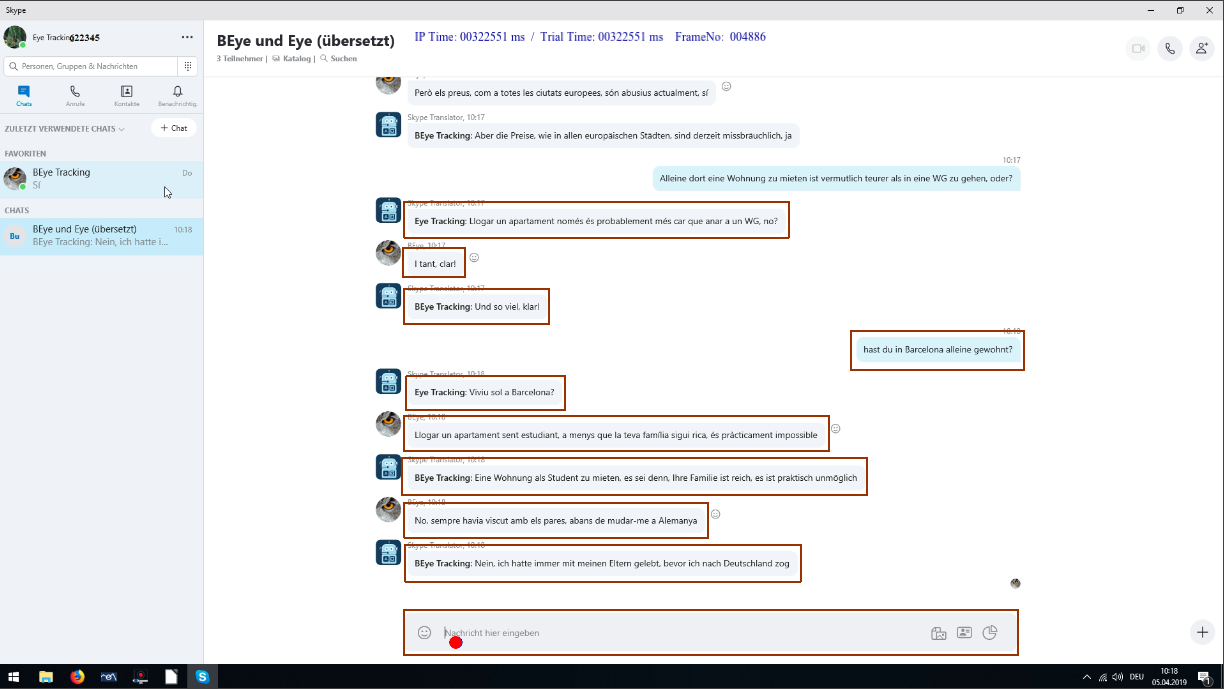
\includegraphics[width=\textwidth]{Figures/EyeTracking/Playback_Image_TN12_TN12_Trial_1.png}
	\caption{Areas of Interest der Feldstudie\label{K5:fig:AOI-Feldstudie}}
\end{figure}


%------------------------------------------------------------------------

%------------------------------------------------------------------------
%%%%%%%%%%%%%%%%%%%%%%%%%%%
%
%
\subsubsection{Einsatz von Eye-Tracking zur MÜ-Evaluation}
\label{K5:subsec:EyeTracking-MüEva}

%------------------------------------------------------------------------

Der Einsatz von Eye-Tracking-Methoden zur Evaluation der MÜ-Qualität ist besonders in Verbindung mit dem Postediting ein kleines, jedoch reges Forschungsfeld. Die MÜ-Ausgabe wird dabei aus unterschiedlichen Blickwinkeln untersucht. Die Wahrnehmung der einzelnen MÜ-Systeme ist ebenso Gegenstand der Untersuchungen wie das Leseverhalten entlang der MÜ-Ausgabe und die Wahrnehmung von Fehlern im rohen Output durch Posteditor{\textperiodcentered}innen. Daher ergeben sich besonders aus diesem Bereich wichtige Anhaltspunkte für die Ausarbeitung der Eye-Tracking-Studie.

Die zweiphasige Studie von \citet[]{doherty_user-based_2012} wird weithin als erste angesehen, die Eye-Tracking zur Untersuchung der Nutzbarkeit von übersetzten Texten durch den/die Endnutzer{\textperiodcentered}in verwendet. Hierzu wurde die Nutzbarkeit der rohen MÜ-Ausgabe auf Deutsch, Französisch, Japanisch und Spanisch mit der des englischsprachigen Originaltextes verglichen. Die Ergebnisse deuten darauf hin, dass wesentliche Unterschiede in puncto Zufriedenheit, Effizient und Zielführung bestehen, abhängig davon, ob Nutzer{\textperiodcentered}innen das Original oder eine MÜ verwenden. In der zweiten Phase der Studie griffen \citet[]{doherty_assessing_2014} die Ergebnisse auf und untersuchten diese auf den Grad der kognitiven Auslastung bei der Verwendung von Original und MÜ. Die Erkenntnisse dieses Studienteils deuten darauf hin, dass die rohe MÜ kognitiv fordernder ist und als weniger nützlich wahrgenommen wird als der Originaltext.

\begin{sloppypar}
\citet[14]{doherty_assessing_2014} befürworten in diesem Zusammenhang explizit den Einsatz von Eye-Tracking-Methoden zur Evaluierung\is{Evaluation} von MÜ-Systemen. Eye-Tracking-Ansätze vermögen es, unbewusste und individuelle kognitive Prozesse der Probanden weitaus deutlicher abzubilden als ähnliche, ebenfalls häufig verwendete Methoden wie Think-Aloud-Protokolle\is{Think-Aloud-Protokoll} oder stimulierte Post-Studien-Interviews\is{Post-Studien-Interview}.\end{sloppypar}

\citeauthor{sajjad_eyes_2016} befassen sich mit dem Leseverhalten bei der Bewertung von maschineller Übersetzung\is{maschinelle Übersetzung}. Die Hypothese ist es, dass eine qualitativ gute MÜ-Ausgabe weitaus weniger kognitiven Aufwand erfordert als schlechte. Dabei folgen die Autoren der Annahme, das Leseverhalten von der Komplexität der syntaktischen Strukturen und der Schwierigkeit des Satzes abhängt. Die Studie greift dabei auf Datenmaterial des WMT’16-Evaluation-Task innerhalb des Sprachenpaares Spanisch-Englisch zurück. 60 mittellange Sätze wurden ausgewählt und von mindestens zwei Annotatoren bewertet. Die jeweils beste und schlechteste Übersetzung wurde mit einem Score (\emph{expected wins}) versehen. So entstanden 120 Evaluationsaufgaben, jeweils 60 gute und 60 schlechte Übersetzungen zu überprüfen. Diese wurden von jeweils sechs Revisor{\textperiodcentered}innen bewertet \citep[1084]{sajjad_eyes_2016}. Zur Untersuchung wählten \citeauthor{sajjad_eyes_2016} die Indikatoren \emph{Verweildauer}\is{Verweildauer}, \emph{Sakkadenanzahl}\is{Sakkadenlänge}\is{Sakkade}, jeweils als \emph{Progressionen}\is{Progression} sowie \emph{Regressionen}\is{Regression}, und die Sakkadenrichtung\is{Sakkadenrichtung} \citep[1083]{sajjad_eyes_2016}. \citeauthor{sajjad_eyes_2016} kommen zu dem Ergebnis, dass sich eindeutige Blickmuster in der Art erkennen lassen, wie die Revisor{\textperiodcentered}innen bei der Bewertung der MÜ-Ausgabe vorgehen.

Die Studie von \citet[]{klerke_reading_2015} untersucht unter Einsatz von Eye-Track\-ing-Methoden das Problemlösungsverhalten von Proband{\textperiodcentered}innen, die Logiktests in der Ausgangssprache, als MÜ-Version, in einfacher Sprache oder als MÜ-Ver\-sion in vereinfachter Sprache bearbeiten sollen. Dabei wird einerseits eine höhere Anzahl an Fixationen sowie eine längere Verweildauer auf der maschinell übersetzten Version beobachtet als auf dem Original. Andererseits lösen die Proband{\textperiodcentered}innen die MÜ-Aufgabe weniger effizient als das Original. Die vereinfachte und maschinell übersetzte Version jedoch scheint diesen Effekt aufzuheben.  

\citet[]{castilho_reading_2018} untersuchen in einer Lesestudie unter Einsatz des Eye-Trackers die qualitative Wahrnehmung der Ausgabe verschiedener MÜ-Systeme. Hierzu dient weiterhin die Bewertung der Zufriedenheit mit dem gelesenen Text und ein Fragebogen zum Leseverständnis. Die Pilotstudie arbeitet mit insgesamt sechs Proband{\textperiodcentered}innen mit Englisch, Spanisch oder Chinesisch als Muttersprache. Die Versuchspersonen sollen die englischsprachigen Ausgangstexte oder die Ausgabe auf Spanisch oder Chinesisch jeweils eines SMÜ- bzw. eines NMÜ-Systems in ihrer Muttersprache lesen. \citeauthor{castilho_reading_2018} kommen zu dem Schluss, dass die NMÜ-Ausgabe zwar zufriedenstellendere Ergebnisse als die der SMÜ für die Versuchspersonen liefert. Die kognitive Auslastung bei der Erfassung ist jedoch für beide Systeme ähnlich.

\citet[]{vardaro_translation_2019} wiederum untersuchen sowohl mit Eye-Tracking-Me\-tho\-den als auch auf Grundlage einer Korpusanalyse, wie professionelle Übersetzungsexpert{\textperiodcentered}innen\footnote{Eng.: \emph{translation expert} -- In der Studie verwendete Sammelbezeichnung für eine Tätigkeit, die sowohl Übersetzung, Postediting als auch Revision umfasst.} der Generaldirekton Übersetzung des Europäischen Parlaments Fehler in der NMÜ sowie der entsprechenden posteditierten Version identifizieren und korrigieren. Die 30 Proband{\textperiodcentered}innen weisen dabei eine hohe fremdsprachliche Kompetenz mit bis zu sechs verschiedenen Ausgangssprachen auf \citep[10]{vardaro_translation_2019}. Zur Identifikation und Korrektur der MÜ-Fehler werden diese in zwei grundlegende Klassen eingeteilt. Unter den Lesefluss betreffende Aspekte (\emph{fluency}) werden Ortographie-, Grammatik-, Konsistenz- sowie Kohärenzfehler gezählt. Die Angemessenheit (\emph{accuracy}) wird durch Sinn- und Auslassungsfehler gekennzeichnet. Die Fehler in der maschinellen Übersetzung wurden auf Grundlage des automatischen Fehlerannotationswerkzeugs \emph{Hjerson} sowie der manuellen \emph{MQM} annotiert. Die Eye-Tracking-Studie erhebt die Dauer der ersten Fixation, die Dauer des ersten Durchlaufs, die regressive Durchlaufdauer sowie die Verweildauer auf dem jeweiligen Ausgangstoken und auf dem Zieltoken. 
Die zentrale Erkenntnis der Studie ist, dass die sprachlich umfassend versierten Versuchspersonen jegliche MÜ-Fehler gleichermaßen schnell identifizieren und keiner Fehlerkategorie Priorität einräumen. Weiterhin scheinen die Versuchspersonen ihre Lese- bzw. Korrekturstrategien den Erfordernissen der jeweiligen Situation anzupassen.
\is{Eye-Tracking|)}


%------------------------------------------------------------------------

\subsection{Konzept der Online-Umfrage}

\label{K5:subsec:Konzept-Umfrage}

%------------------------------------------------------------------------


Mit der Umfrage sollen zunächst aktuelle Daten zum Nutzerkreis, zum Nutzungsverhalten und -- mit Fokus auf dem Skype Translator\is{Skype!Skype Translator} -- zum Kenntnisstand im Umgang mit dieser Technologie erhoben werden. Diese aktuellen Daten sollen eine Zuarbeit für die anschließende Feldstudie mit dem Skype Translator liefern, die in \ref{K5:subsec:Konzept-Feldstudie} (S.\,\pageref{K5:subsec:Konzept-Feldstudie}) genau beschrieben wird. Eine Interviewsituation, sowohl strukturiert als auch semi-strukturiert, wurde als Möglichkeit der Erhebung verworfen, da der zeitliche Aufwand in keiner Relation zu der benötigten Teilnehmerzahl und den erwarteten Antworten steht und somit schlichtweg kaum durchführbar ist.

Mit Blick auf den intendierten Proband{\textperiodcentered}innenkreis der Feldstudie um den Skype Translator\is{Skype!Skype Translator} wurde als Zielgruppe für die Umfrage das gleiche Umfeld ausgewählt: Student{\textperiodcentered}innen jeglicher Fachrichtung an deutschen Universitäten. Um eine möglichst weitläufige Stichprobe zu ziehen, wurde der Fragebogen\is{Fragebogen} als Online-Version\is{Umfrage!online} über Verteilerlisten an Universitäten in Deutschland versendet und als Link in entsprechenden Hochschulgruppen\footnote{Gerade zu Beginn des jeweiligen akademischen Jahres, also dann, wenn neue Erstsemester an die Universitäten drängen, sind die umgangssprachlich als \emph{Ersti-Gruppen} bezeichneten Gemeinschaften auf Facebook ein guter Anlaufpunkt für die Verbreitung von derartigen Umfragen. Dies hängt jedoch auch in großen Teilen vom Wohlwollen der Administratoren ab.} innerhalb von Facebook verbreitet. \citeauthor{aeppli_empirisches_2016} sprechen in diesem Fall von einer Klumpenstichprobe, die auf \glqq natürlich vorkommende Gruppen\grqq{} \citep[174]{aeppli_empirisches_2016} abzielt. Das einzige einschränkende Kriterium ist die Verwendung von Skype\is{Skype}, wobei auch die Verwendung des Internets zum Zwecke der Diffusion des Fragebogens als Zugangsbarriere angesehen werden kann \citep[174]{aeppli_empirisches_2016}. Allerdings kann dieses Manko insofern vernachlässigt werden, als für die Nutzung von Skype ohnehin ein Internetzugang bestehen muss.

Ein generelles Problem bei Online-Umfragen\is{Umfrage!online} stellt jedoch die Zugangsbegrenzung bzw. die zielgruppengenaue Veröffentlichung dar. Dies wird sowohl mit Blick auf die Altersangaben der Teilnehmer{\textperiodcentered}innen, den höchsten Abschluss als auch die Auslandserfahrung deutlich. Die genauen Angaben zu diesen Fragen sind im Abschnitt~\ref{K6:subsec:Ergebnisse-Umfrage} (S.\,\pageref{K6:subsec:Ergebnisse-Umfrage}) detailliert offengelegt. Hierbei ist allerdings zu erwähnen, dass auch Institutionen, die keine Rückmeldung auf die Anfrage zur Verbreitung des Fragebogens gegeben haben, dennoch den Aufruf über entsprechende Verteilerlisten veröffentlicht haben. Diese -- zugegebenermaßen vage -- Annahme basiert auf dem Teilnahmezähler des verwendeten Online-Tools.

Der Fragebogen\is{Fragebogen} für diese Arbeit konzipierte Fragebogen umfasst insgesamt 38 Items. Die Erhebung findet dabei sowohl in Form von Ja-Nein-Fragen (z.\,B.\ S.\,\pageref{App1:freq}), offenen Fragen mit Freitextfeldern als auch geschlossenen Fragen mit Mehrfachantworten (z.\,B.\ S.\,\pageref{App1:Alt}) oder Skalen (z.\,B.\ S.\,\pageref{App1:NST}) statt \citep[138\psq]{atteslander_methoden_2010}. Die Skalen umfassen eine Abstufung von 1--4, was sprachlich mit Oppositionspaaren unterstützt wird. Es wurde bewusst eine geringe Spanne ohne Mittelwert gewählt, um so wenig aussagekräftige, unentschlossene Antworten zu vermeiden und die Teilnehmer{\textperiodcentered}innen zu einer positionierten Aussage zu bewegen. Weiterhin sind die Items des Fragebogens in sechs Unterthemen aufgeteilt:\is{Skype|(} \emph{Nutzung von Skype} (S.\,\pageref{App1:SectionNutzung}), \emph{Nutzungsbewertung} (S.\,\pageref{App1:SectionNutzungsbewerung}), \emph{Nutzungsbewertung Skype Translator} (S.\,\pageref{App1:SectionNutzungsbewerungST}), \emph{Alternativen} (S.\,\pageref{App1:SectionAlternativen}), \emph{Auslandeserfahrung -- gegenwärtig \& vergangen} (S.\,\pageref{App1:SectionAuslandserfahrung}) und \emph{individuelle Angaben} (S.\,\pageref{App1:SectionDemographie}). Alle Fragetypen sind so eingestellt, dass dem Teilnehmer{\textperiodcentered}innen auch die Möglichkeit geboten wurde, sich entweder komplett der Beantwortung zu verweigern oder zumindest keine Angaben zu machen. Ebenfalls war es möglich, die Eingangsfrage \emph{Nutzen Sie Skype?} mit \emph{Nein} zu beantworten. In diesem Falle wurde die Online-Umfrage so konditioniert, alle weiteren Fragen, die in direktem Zusammenhang mit Skype stehen, zu überspringen und sogleich zu den weiteren Aspekten zu leiten.

Im Umfrageteil zur generellen Nutzung von Skype werden konkret Nutzungsdauer, -länge, -modus, sowie die Skypeversion und die Art der Gesprächspartner{\textperiodcentered}innen erhoben. Neben einem Freitextfeld zur Angabe weiterer Anwendungen führt der Umfrageteil zur Nutzung von Alternativen folgende Dienste auf: \emph{Appear.in}\is{Appear.in}, \emph{Facebook Messenger}\is{Facebook!Messenger}\is{Facebook Messenger}, \emph{Google Hangouts}\is{Google!Hangouts}\is{Google Hangouts}, \emph{Apple Facetime}\is{Apple!Facetime}\is{Apple Facetime}, \emph{WhatsApp}\is{WhatsApp}, \emph{Telegram}\is{Telegram}, \emph{Viber}\is{Viber}, \emph{Twitter}\is{Twitter}, \emph{Snapchat}\is{Twitter}, \emph{Instagram-Chat}\is{Instagram}\is{Facebook!Instagram} und \emph{ICQ}\is{ICQ}. Die Auswahl dieser Anwendungen erfolgte dabei aufgrund des Bekanntheitsgrades und wurde großzügig weit gefasst, um Umfrageteilnehmer{\textperiodcentered}innen nicht durch eine zu begrenzte Auswahl auf \emph{Skype} zu fokussieren. Zusätzlich zur generellen Nutzung der angebotenen Alternativen wurde ebenfalls nach der am häufigsten verwendeten Software -- unterschieden nach Modus Video-\is{Chat!Video-}, Voice-\is{Chat!Voice-} und Textchat\is{Chat!Text-} -- gefragt.\is{Skype|)}

Im Bereich der Auslandserfahrung wurde zwischen gegenwärtigen und vergangenen Reisen unterschieden. Als Auslandserfahrung wurden dabei Aufenthalte definiert, die einerseits keinen Urlaub darstellten und andererseits länger als vier Wochen dauerten. Somit sollte sichergestellt werden, dass die Umfrageteilnehmer{\textperiodcentered}innen eindeutig einen Landes- und Sprachkontakt nachweisen konnten. Die Unterscheidung zwischen gegenwärtig und vergangen wurde vorgenommen, da aufgrund der intendierten Zielgruppe nicht ausgeschlossen werden konnte, ob Studierende den Aufruf zur Teilnahme im Laufe ihres Auslandsaufenthaltes erhielten. Neben der Frage nach dem Grund der Reise -- \emph{Spracherwerb}, \emph{Sprachvertiefung}, \emph{Kulturkontakt}, \emph{Pflichtaufenthalt}, \emph{Fortbildung}, \emph{beruflich} und  \emph{sonstiges} -- wurde das Land, der (schwerpunktmäßige) Hauptaufenthaltsort sowie die Dauer in Monaten erhoben.

Im Rahmen der demographischen Angaben wurden das Geschlecht, das Alter und der höchste Abschluss (\emph{kein Abschluss}, \emph{bis mittlere Reife}, \emph{Hochschulzugangsberechtigung}, \emph{abgeschlossene Ausbildung}, \emph{höherer Berufsabschluss}, \emph{Hochschulabschluss} sowie \emph{sonstiges}) erhoben. Auch die Sprachkenntnisse der Teilnehmer{\textperiodcentered}\linebreak[3]innen wurde abgefragt. Dies geschah aufgeteilt nach Sprachen, mit denen man primär aufgewachsen war, die man hauptsächlich im Alltag und hauptsächlich im Beruf verwendete. Eine Selbsteinschätzung erhob abschließend die Kompetenz gemäß des Europäischen Referenzrahmens für die Sprachen Spanisch, Katalanisch, Galicisch, Portugiesisch, Italienisch, Französisch und Rumänisch, wobei die Teilnehmer{\textperiodcentered}innen nur Angaben machen sollten, sofern sie eine nachweisliche Qualifikation (Zeugnis, Zertifikat o.\,ä.) hierrüber besaßen.

%------------------------------------------------------------------------

\subsection{Datenschutz und Anonymität} 
\label{K5:subsec:Anonymitaet}

%------------------------------------------------------------------------

Die Verbreitung und Bearbeitung dieses Fragebogens erfolgen ausschließlich online. Daher enthält die hier abgedruckte Fassung zwar Fragen zur Person, jedoch keine Elemente wie sie bei einer manuellen Aufbereitung notwendig sind, so z.\,B.\ die anonymisierten Teilnahmecodes oder fortlaufende Ziffern zur Systematisierung. Die Anonymisierung erfolgt durch das verwendete Online-Umfragetool der Universität Leipzig auf Basis von \emph{LimeSurvey}\footnote{Verwendet in der Version 3.22.27+200720.}. Unabhängig von der eigens ausgearbeiteten Eingangsbelehrung weist auch das Onlinewerkzeug auf geltende Datenschutzrichtlinien hin (s. Anhang \ref{App1:HinweisLimeSurvey}, S.\,\pageref{App1:HinweisLimeSurvey}).

Zusätzlich wurde ein individueller Hinweis auf die Teilnahmebedingungen der Umfrage ausgearbeitet. Dieser wird, ebenso wie die Angaben zum Untersuchungsvorhaben und eine Anleitung, vor Beginn der Online-Umfrage eingeblendet (s. Anhang \ref{App1:HinweisIndiv}, S.\,\pageref{App1:HinweisIndiv}).

%------------------------------------------------------------------------

\subsection{Konzept der Feldstudie}
\label{K5:subsec:Konzept-Feldstudie}

%------------------------------------------------------------------------

Die Feldstudie fand in den Räumlichkeiten des IALT statt. \citet[263]{obrien_eye_2009} empfiehlt für optimale Versuchsbedingungen die Nutzung eines Eye-Tracking-Labors\is{Eye-Tracking!-Labor}, in dem die Lichtverhältnisse kontrolliert werden können. Da es am IALT zum Zeitpunkt dieser Arbeit noch kein solches Labor gab, wurde ein gewöhnlicher Büroraum genutzt. Um dennoch die Lichtverhältnisse kontrollieren zu können, wurde jede Sitzung mit heruntergelassenen Sonnenblenden und bei eingeschalteter Deckenlampe durchgeführt.

Der Eye-Tracker, der dabei verwendet wurde, war der \emph{Eye Link Portable Duo} von SR Research. Der gesamte Aufbau besteht aus einem \emph{Display-PC}, einem \emph{Host-PC} und der Eye-Tracking-Kamera. Erster enthält eine gewöhnliche Windows-Distribution, Skype und die Software zur Bildschirmaufnahme. Über ein LAN-Kabel ist der Display-PC mit dem Host-PC verbunden, von dem aus der Eye-Tracker gesteuert werden kann. Neben Tastatur und Maus wurden keine weiteren peripheren Eingabegeräte verwendet. Für die Durchführung wurde der Eye-Tracker\is{Eye-Tracking!-Modus} im freien Modus (sog. \emph{head-free-to-move mode}) verwendet, bei dem die Kamera zwischen Bildschirm und Tastatur auf einem Tripoden platziert wird. Bei dieser Einstellung ist es nicht nötig, den Kopf der Proband{\textperiodcentered}innen zu fixieren. Ein Sticker in Form einer kleinen Zielscheibe auf der Stirn der Person reicht dem System aus, um die Augen zu triangulieren. Eine Kalibrierung des Systems auf die jeweilige Person ist jedoch weiterhin erforderlich. Als Bildwiederholungsrate wurde mit 1.000\,Hz der höchstmögliche Wert im freien Modus gewählt. Dabei zeichnete das System die Bewegungen beider Augen auf (\emph{binocular recording})\is{binocular recording|see{Eye-Tracking}}, nachdem eine 9-Punkt-Kalibrierung durchgeführt wurde. Die Abbildung~\ref{K5:fig:Skizze-Vogelperspektive} (S.\,\pageref{K5:fig:Skizze-Vogelperspektive}) skizziert den Versuchsaufbau aus der Vogelperspektive. Der Versuchsleiter und die jeweilige Versuchsperson saßen sich gegenüber. Das gesamte Eye-Tracking-Equipment befand sich ebenfalls auf dem Bürotisch zwischen beiden Personen. Der Versuchsleiter konnte nur die Ausgabe des Host-PCs sehen. Die Versuchsperson hatte wiederum nur Sicht auf den Display-PC.

%------------------------------------------------------------------------

\begin{figure}
    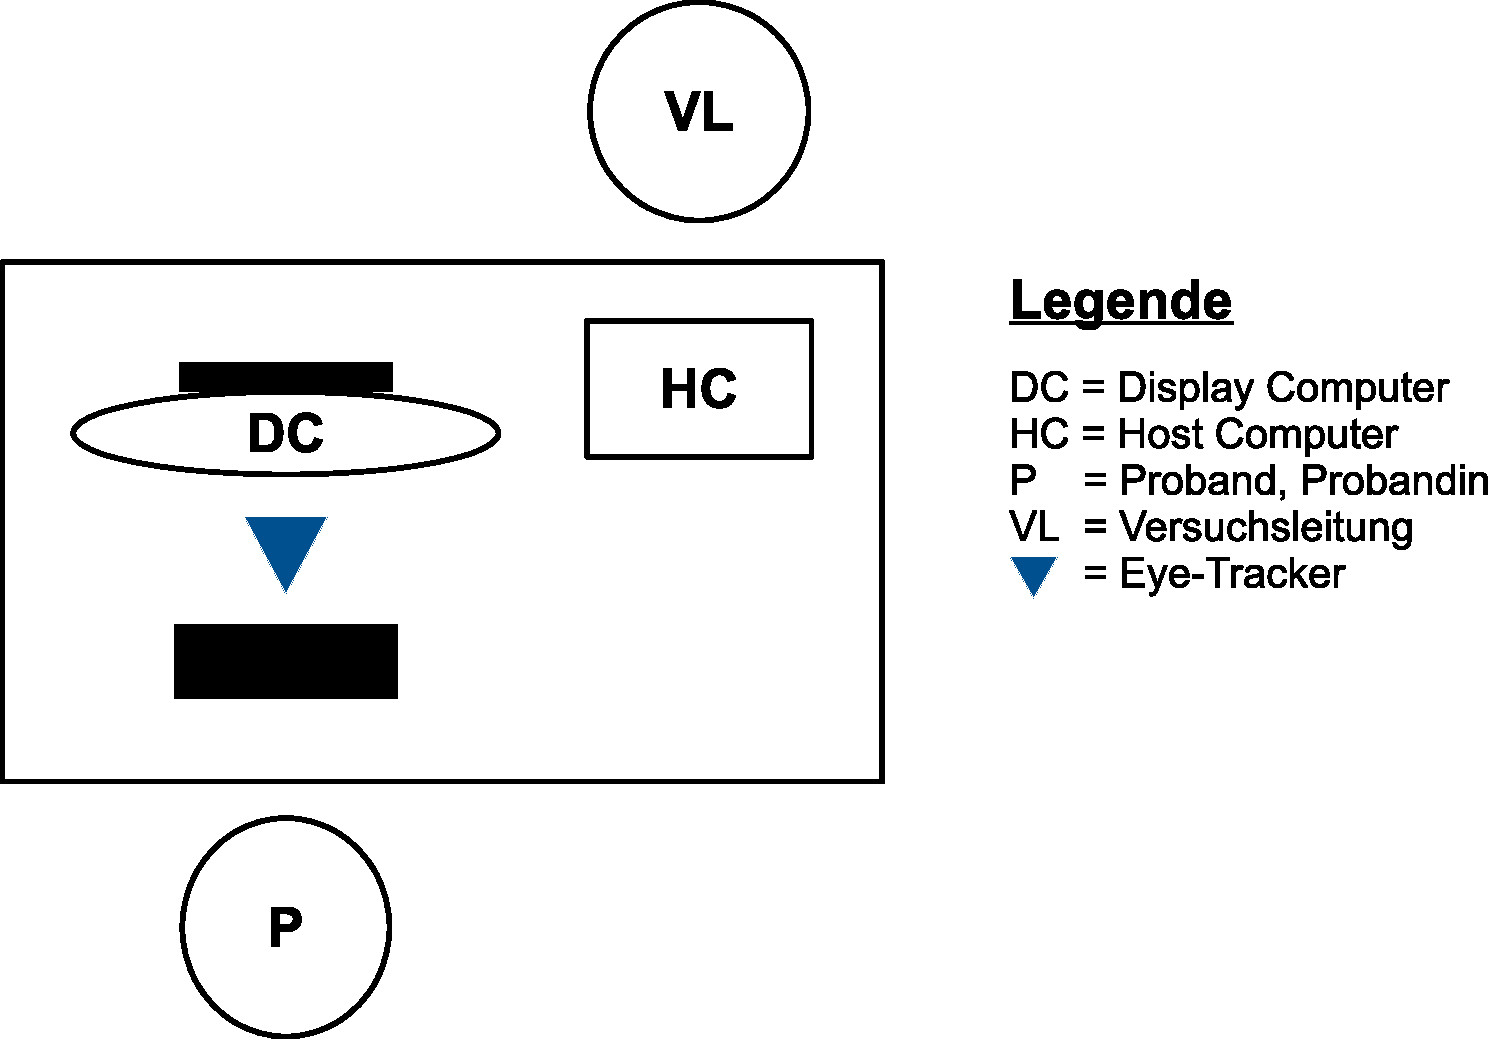
\includegraphics[width=9cm]{Figures/EyeTracking/skizze-versuchsaufbau-vogelperspektive.pdf}
	\caption{Versuchsaufbau aus der Vogelperspektive\label{K5:fig:Skizze-Vogelperspektive}}
\end{figure}


%------------------------------------------------------

\citet[240]{balling_evidence_2014} weisen darauf hin, dass die gegebene Bewegungsfreiheit der Proband{\textperiodcentered}innen im gewählten freien Aufnahmemodus zu Präzisionsverlusten bei der Erfassung der Augenbewegung führen kann. Eine mögliche Lösung wäre die Nutzung einer Kinnstütze, die jedoch den Bewegungsradius der Versuchsperson einschränkt. Im Rahmen der naturalistisch orientierten Translationsprozessforschung ist von diesem Vorgehen daher abzuraten.

Für die Studie wurde mit der jeweils aktuellsten Skype-Version\is{Skype!-Version} für Windows 10 gearbeitet. Die Bildschirmaufnahmen und die Datenaufbereitung wurde mit proprietärer Software von SR Research durchgeführt. Die Mitschnitte der einzelnen Sitzungen liegen im MP4-Format vor. Außerdem registrierte das System neben den Augenbewegungen auch alle Eingabesignale der Peripheriegeräte. Diese \emph{Key-Logs}\is{Key Logging} können für weitere Untersuchungen an den Daten verwendet werden.

Die proprietäre Software \emph{SR Research Data Viewer}\footnote{Verwendet in der Version 4.1.1.} ermöglichte die Aufbereitung der gesammelten Rohdaten. Ohne vorherige Bearbeitung liefert die Software bereits sog. \emph{Heatmaps}\is{Heatmap} und Screenshots zu den Fixationen\is{Fixation}, Sakkaden\is{Sakkade} und Blinzlern\is{Blinzler}. Eine kombinierte Ansicht aus den Events und allen Eingabesignalen ist ebenfalls möglich. Darüber hinaus liefert die Betrachtung der Rohdaten Angaben zu den grundlegenden Einstellungen der Aufnahme, wie etwa Bildschirmgröße in Pixeln, Sitzungsdauer, verwendeter Modus des Eye-Trackers usw.

Es ist weiterhin möglich, statische Stimuli\is{Stimulus} automatisch mit AOI versehen zu lassen. Dies ist bei der Aufbereitung von Texten oder Bildern hilfreich. Bei Bildschirmmitschnitten mit häufigen Positionswechseln der AOI, wie etwa bei der Feldstudie dieser Arbeit (s. hierzu die Abbildungen\,\ref{K3:fig:Ausschnitt-Ausgabe-MT-ST}, S.\,\pageref{K3:fig:Ausschnitt-Ausgabe-MT-ST} und \ref{K5:fig:AOI-Feldstudie}, S.\,\pageref{K5:fig:AOI-Feldstudie}), mussten die Rohdaten zunächst manuell annotiert werden. Dabei wurde mit fünf Kategorien an statischen\is{Area of Interest!statisches} und dynamischen AOI\is{Area of Interest!dynamisches} (s. hierzu S.\,\pageref{K5:subsubsec:DynAOI}) gearbeitet: Die Eingabemaske des Skype Translators wurde als statisches AOI mit dem Label \emph{Eingabe} versehen. In den Rohdaten wurden originale, deutschsprachige Chatbeiträge\is{Chat!-beitrag} der/des Proband{\textperiodcentered}in zunächst mit dem fortlaufend nummerierten Label \emph{AEyeO-\#} erfasst, die entsprechende katalanische maschinelle Übersetzung mit \emph{AEyeMT-\#}. Die Beiträge des katalanischsprachigen Gegenübers erhielten respektive hierzu die Marken \emph{BEyeO-\#} und \emph{BEyeMT-\#}. Um für die Analyse eine eindeutige Grundlage mit Blick auf Übersetzungsrichtung und Sprache zu schaffen, wurden die Labels im Zuge der Auswertung gemäß der Länderkürzel der ISO-639-1\footnote{S. hierzu \url{https://www.bib-bvb.de/web/kkb-online/rda-sprachencode-nach-iso-639}, Abruf am \datum{}.} abgeändert. Dementsprechend finden sich in dieser Arbeit nun die Labels \label{K5:itemize:labelnamen}

\begin{description}[font=\normalfont\scshape]
    \item [GerO] für den originalen, deutschsprachigen Beitrag der Versuchsperson,
    \item [CatMT] für die maschinelle Übersetzung ins Katalanische, 
    \item [CatO] für den originalen, katalanischsprachigen Beitrag des Gegenübers und
    \item [GerMT] für die maschinelle Übersetzung ins Deutsche
\end{description}
für die dynamischen AOI\is{Area of Interest!dynamisches} im Setting Katalanisch-Deutsch und

\begin{description}[font=\normalfont]
    \item[A] für die originalen, deutschsprachigen Beiträge der Versuchsperson,
    \item[B] für die originalen, deutschsprachigen Beiträge des Gegenübers 
\end{description}
für die dynamischen AOI im Setting Deutsch-Deutsch.

Bei der Annotation wurden die Chatbeiträge\is{Chat!-beitrag} dabei bis zu einer Höhe von etwa zwei Drittel der Bildschirmanzeige mit dynamischen AOI\is{Area of Interest!dynamisches} versehen, da die Mehrheit der Eye-Tracking-Events sich hauptsächlich in diesem Bereich verteilte. Dies wird in der Darstellung als Heatmap \is{Heatmap} deutlich, wie \figref{K5:fig:Heatmap-TN24} (S.\,\pageref{K5:fig:Heatmap-TN24}) zeigt. Als weiteren Beleg für die Annotation bis zu einer Höhe von zwei Dritteln des Bildschirms dient die graphische Darstellung der Fixationen\is{Fixation}, Sakkaden\is{Sakkade} und Blinzler\is{Blinzler} jeweils für beide Studienversionen in den Abschnitten \ref{K6:sub:catde:graph-inspect} (S.\,\pageref{K6:sub:catde:graph-inspect}) und \ref{K6:sub:dede:graph-inspect} (S.\,\pageref{K6:sub:dede:graph-inspect}). Gemessen an den Hinweisen von \citeauthor{obrien_eye_2009} (s. in dieser Arbeit Kap.\,\ref{K5:subsubsec:DynAOI}, S.\,\pageref{K5:subsubsec:DynAOI}), kann die vorliegende Studie keine Analyse auf Wortebene liefern, da die Auflösung des Bildschirms und die Standard-Schriftgröße des Chats bei Skype\is{Skype}\is{Chat!Text-} zu klein für eine sinnvolle Annotation von AOI entlang der Wortgrenzen ist.

%------------------------------------------------------------------------

\begin{figure}
    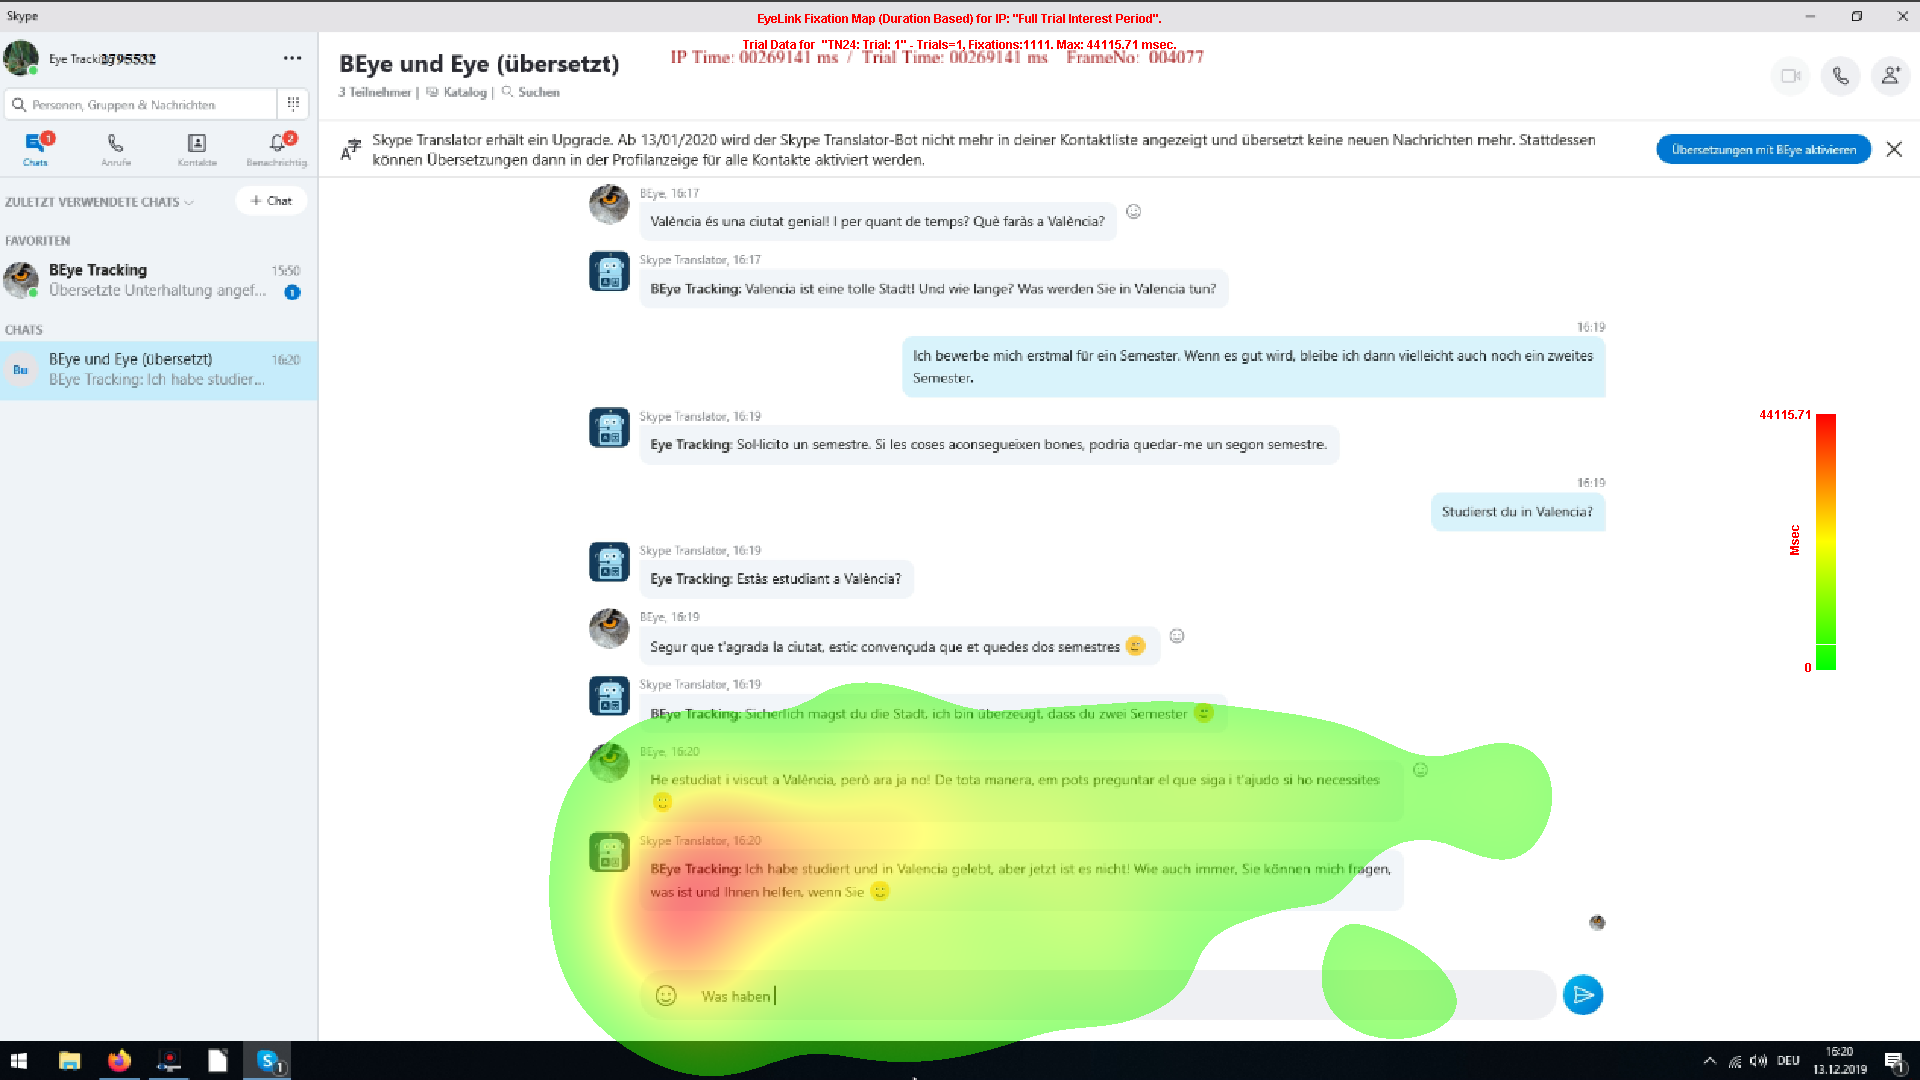
\includegraphics[width=\textwidth]{Figures/Fixmaps/CatDe/Fixmap_TN24_Trial_1.png}
	\caption{Heatmap einer Bildschirmaufnahme\label{K5:fig:Heatmap-TN24}}
\end{figure}


%------------------------------------------------------------------------


Da mit zwei Versuchsgruppen und sich leicht voneinander unterscheidenden Abläufen gearbeitet wurde, werden die grundlegenden Informationen zu den Kohorten im jeweiligen Abschnitt -- für das Setting Katalanisch-Deutsch ab S.\,\pageref{K6:subsec:Angaben-Eingang-Probandinnen-CatDe} und für das Setting Deutsch-Deutsch ab S.\,\pageref{K6:subsec:Angaben-Eingang-Probandinnen-DeDe} -- dargelegt.

%%%%%%%%%%%%%%%%%
% Auf Anraten von Christine noch genauer das Setting beschreiben. Ggf. auf Koch/österreicher kritisch verweisen, aber die Situation einordnen, wieso das ganze im Büro stattfand und welche Parameter dabei noch zu beachten waren
%%%%%%%%%%%%%%%%%

%------------------------------------------------------------------------

\section{Die Feldstudie}

\label{K5:sec:Feldstudie}

%------------------------------------------------------------------------

Die Feldstudie wurde in zwei Settings mit sich nicht überschneidenden Teilnehmer{\textperiodcentered}innengruppen und einem mehrteiligen Aufbau durchgeführt. Eine Variante sah den Textchat\is{Chat!Text-} von deutschen Muttersprachlern mit katalanischen Muttersprachlern über Skype\is{Skype!Skype Translator} und bei aktiviertem Skype Translator vor, wobei die deutsche Seite mit einem Eye-Tracking-System\is{Eye-Tracking} erfasst und ein Videomitschnitt der Bildschirmaktivität (eng.: \emph{screen recording}) erzeugt wurde.

\begin{sloppypar}
Diese Gesprächssituation war flankiert von einem digitalen Eingangs- und einem Ausgangsfragebogen\is{Fragebogen}, die die Versuchspersonen zu beantworten hatten, und deren Ergebnisse im weiteren Verlauf dieser Arbeit vorgestellt werden.
Der Ablauf dieser Studienvariante kann daher wie folgt skizziert werden: Die Proband{\textperiodcentered}innen wurden zunächst gebeten, den Eingangsfragebogen (s. Abschnitt \ref{K6:subsec:Angaben-Eingang-Probandinnen-CatDe}, S.\,\pageref{K6:subsec:Angaben-Eingang-Probandinnen-CatDe}, und Anhang \ref{App:F2}, S.\,\pageref{App:F2}) zum Kenntnisstand im Umgang mit Skype und zur eigenen Auslandserfahrung auszufüllen. Dann folgte der aufgezeichnete Textchat über Skype bei aktiviertem Skype Translator. Danach erhielten die Proband{\textperiodcentered}innen den Ausgangsfragebogen (s. Anhang\,\ref{App3:F3}, S.\,\pageref{App3:F3}), der Angaben zur Nutzungserfahrung erheben sollte. Die Ergebnisse dieses Ausgangsfragebogens werden ab Kapitel\,\ref{K6:sub:Ausgangsfragebogen:CatDe}, Seite\,\pageref{K6:sub:Ausgangsfragebogen:CatDe} betrachtet. 
\end{sloppypar}

Die zweite Studienvariante sah Textchats\is{Chat!Text-} von deutschen Muttersprachlern untereinander über Skype vor. Auch hier kamen das Eye-Tracking-System sowie die Bildschirmaufzeichnung zum Einsatz. Die Proband{\textperiodcentered}innen erhielten bei dieser Variante jedoch nur den Eingangsfragebogen (s. Anhang\,\ref{App:F2}, S.\,\pageref{App:F2}). Dieser Aufbau diente dem Vergleich. Ein monolinguale Durchführung ohne den zentralen Stimulus\is{Stimulus}, den die maschinelle Übersetzung\is{maschinelle Übersetzung} des Skype Translators\is{Skype!Skype Translator} liefert, sollte daher Aufschluss über das Nutzer{\textperiodcentered}innenverhalten in einem reinen Chat-Gespräch\is{Chat} geben.


%------------------------------------------------------------------------

\subsection{Abhängige Variablen der statistischen Analyse}
\label{K5:subsubsec:AbhaengigeVariablenStatAna}

%------------------------------------------------------------------------
\begin{sloppypar}
\citet[25]{jakobsen_reading_2017} weisen darauf hin, dass man die Variablen einer kognitionwissenschaftlichen Studie auf zwei Arten kontrollieren kann: Auf natürlichem Wege kann zu Beginn der Studie festgelegt werden, welche Faktoren eine Auswirkung auf die Untersuchungssituation haben. Hierbei muss jedoch von vornherein sicher sein, dass diese Faktoren die Situation zweifelsfrei beeinflussen und welche Auswirkungen zu erwarten sind. Da dies bei Studien mit mehreren Variablen häufig nur kaum bis überhaupt nicht möglich ist, bauen viele Analysen auf dem sog. \emph{linear mixed-effects regression model} auf, einer statistischen Betrachtung der unterschiedlichen Faktoren und ihrer Auswirkung auf eine abhängige Variable. Gegenüber anderen statistischen Methoden\is{Statistik} wie der Varianzanalyse\is{Varianzanalyse|seealso{Statistik}}\is{Statistik!Testverfahren!Varianzanalyse} (\emph{ANOVA})\is{ANOVA|see{Varianzanalyse}} besitzen derartige Regressionsmodelle\is{Regressionsmodell|see{Statistik}}\is{Statistik!Testverfahren!Regressionsmodell} die Eigenschaft, flexibel auf unausgeglichene Daten zu reagieren. So können beispielsweise die individuellen Unterschiede zwischen Proband{\textperiodcentered}innen als Zufallsvariablen kontrolliert werden, die im Rahmen der natürlichen Konzeption nur schwer zu beherrschen sind. Gleichzeitig können fixierte Variablen wie das Geschlecht in das Modell integriert werden. Gerade im Rahmen einer naturalistisch orientieren Translationsprozessforschung\is{Translationsprozessforschung} wird diese statistische Methode\is{Statistik} häufig verwendet \citep[vgl.\,z.\,B.][]{jakobsen_reading_2017, jakobsen_chapter_2017}. Eine Grundvoraussetzung dafür ist jedoch die Annahme der Normalverteilung der Daten. Sollte diese Annahme nicht möglich sein, können sog. nicht-parametrische Tests\is{Statistik!Testverfahren!nicht-parametrisches}\is{nicht-parametrischer Test|see{Statistik}} verwendet werden. Diese stellen ebenfalls gewisse Anforderungen an die Beschaffenheit der Datengrundlage, können aber auch dann eingesetzt werden, wenn die Daten nicht normal verteilt sind. Bei der Analyse in Kapitel \ref{K6} wird deshalb jede verwendete Variable auf ihre Verteilung hin überprüft und das statistische Testverfahren entsprechend gewählt. Um die Bedeutsamkeit des Testergebnisses zu beurteilen, wird bei signifikanten Unterschieden zudem die Effektstärke angegeben. Diese verdeutlicht die praktische Relevanz des Testergebnisses.\end{sloppypar}

\begin{sloppypar}
Die Unterscheidung zwischen unabhängigen und abhängigen Variablen stammt ursprünglich aus der Psychologie, wird jedoch auch bei der Operationalisierung von Eye-Tracking-Variablen verwendet \citep[6]{huang_visual_2014}. Unabhängige Variablen stellen dabei den veränderbaren Teil eines Experiments bzw. einer Hypothese dar, da nur sie vom Forscher beeinflusst und verändert werden können. Abhängige Variablen hingegen zeigen den Effekt, den die Manipulation der unabhängigen Variablen haben. Die Darstellung des Vorgehens zur Messung dieser Effekte inkl. Begriffsdefinition und Angabe der Messverfahren ist die Operationalisierung (\cite[81]{albert_empirisches_2014}, \cite[125\psqq]{aeppli_empirisches_2016}). Soweit möglich und sinnvoll, werden im Folgenden die Variablen mit einer deutschen Bezeichnung aufgeführt. Eine Übernahme der geläufigen englischen Bezeichnungen hätte den Lesefluss gestört. 
\end{sloppypar}

\citet[218]{duchowski_eye_2017} kategorisiert folgende Indikatoren als traditionelle Eye-Tracking-Maße\is{Eye-Tracking!-Indikatoren}:

\begin{itemize}
    \item Fixation inkl. Regressionen\is{Fixation}\is{Regression}
    \item Dauer der Fixation (Fixation Duration)\is{Fixation!Dauer der}
    \item Anzahl an Fixationen (global)\is{Fixation!-sanzahl}
    \item Fixationsrate (global)\is{Fixation!-srate}
    \item durchschnittliche Fixationsdauer (global)\is{Fixation!-sdauer}
    \item Blickverlauf (Fixationssequenz)\is{Fixation!-ssequenz}
    \item Fixierte Anzahl an Area of Interest (AOI)\is{Area of Interest!Anzahl an}
    \item Prozentualer Anteil der Fixation pro AOI\is{Area of Interest!Anteil an}
    \item Anzahl an Fixationen pro AOI (Fixation Count)\is{Area of Interest!Anzahl an Fixationen pro}
    \item durchschnittliche Verweildauer inkl. Sakkaden und Fixationen pro AOI (Dwell Time)\is{Area of Interest!Verweildauer im}
\end{itemize}


Neben diesen Indikatoren werden in Lesestudien ferner Sakkaden\is{Sakkade} und die Pupillengröße\is{Fixation!Pupillengröße} zur Untersuchung herangezogen. Allerdings ist sich die Forschung bei diesen beiden Variablen nicht einig, wie präzise sie die kognitive Auslastung abbilden und wie zuverlässig mögliche Aussagen sind. Aus der Gesamtheit an Maßen werden für die vorliegende Arbeit einzelne Indikatoren ausgewählt und im Kapitel\,\ref{K6:sec:Probandinnen-CatDe} ab Seite\,\pageref{K6:sec:Probandinnen-CatDe} eingehend untersucht. Die Auswahl wurde ausgehend von den in Abschnitt \ref{K5:subsec:EyeTracking-MüEva} (S.\,\pageref{K5:subsec:EyeTracking-MüEva}) kurz umrissenen Studien getroffen, auch wenn darüberhinaus noch weitere Maße (s.\,o., s.\,u.) miteinbezogen werden. Die Definition und Abkürzung ist dabei der Dokumentation der proprietären Analysesoftware von \citet[]{sr_research_ltd_eyelink_2019} entlehnt:

\begin{description}[font=\normalfont]
    \item [Fixationsanzahl ({FixC}):] Anzahl aller Fixationen\is{Fixation!-sanzahl} in einem AOI in absoluten Zahlen
    \item [Dauer der ersten Fixation ({IAFFD})] in einem AOI\is{Fixation!Dauer der ersten}
    \item [Regressionen ({Reg}):] Rückkehr\is{Regression} in ein AOI, wenn zuvor bereits ein AOI höherer Ordnungszahl betreten wurde. Die Variable ist nominalskaliert und besitzt lediglich zwei Zustände: ja (1) und nein (0).
    
        \begin{description}[font=\normalfont]
            \item [Eingangsregression ({RegIn}):] Rückfall in ein AOI\is{Regression!eingehende}
            \item [Ausgangsregression ({RegOut}):] Rückfall aus einem AOI\is{Regression!ausgehende}
        \end{description}
    
    \item [Verweildauer im ersten Durchlauf (IAFRD):] Dauer des ersten\is{first run dwell time|see{Verweildauer im ersten Durchlauf}}\is{Verweildauer im ersten Durchlauf} Durchlaufs in Millisekunden, in Form der Summe aller Fixationen ohne Sakkaden, ab Betreten des AOI bis zum Verlassen hin zu einem AOI höherer Ordnungszahl
    \item [Verweildauer ({Dwell}):] Aufsummierte Dauer aller Fixationen ungeachtet der Sakkaden in einem AOI in Millisekunden
    \item [Regressive Durchlaufdauer ({IARegPD}):] Aufsummierte\is{Durchlauf!-dauer!regressive} Dauer in Millisekunden aller Fixationen innerhalb eines AOI ab dem erstmaligen Betreten bis zum erstmaligen Verlassen hin zu einem AOI höherer Ordnungszahl. Wurden in dieser Zwischenzeit AOI mit niedrigerer Ordnungszahl fixiert, wird auch diese Dauer hinzuaddiert.
        \begin{description}[font=\normalfont]
            \item [Selektive regressive Durchlaufdauer (IASelRegPD):] Aufsummierte Dauer\is{Durchlauf!-dauer!selektive regressive} in Millisekunden aller Fixationen innerhalb eines AOI ab dem erstmaligen Betreten bis zum erstmaligen Verlassen hin zu einem AOI höherer Ordnungszahl, ohne die Dauer der Fixationen, die in dieser Zwischenzeit in AOI mit niedrigerer Ordnungszahl verbracht wurde
        \end{description}
    \item [Sakkadenamplitude (SacAmp):] Größe der gegenwärtigen Sakkade,\is{Sakkade!-namplitude} angegeben in Grad des sichtbaren Winkels (\emph{degrees of visual angle})
    \item [Sakkadendauer (SacDur):] Dauer der gegenwärtigen \is{Sakkade!-ndauer}Sakkade, angegeben in Millisekunden
    \item [Pupillengröße (PSize):] Pupillengröße\is{Fixation!Pupillengröße} in willkürlichen Einheiten (\emph{arbitrary units})
\end{description}

%------------------------------------------------------------------------

\subsection{Unabhängige Variablen der statistischen Analyse}
\label{K5:subsubsec:UnabhaengigeVariablenStudie}

%------------------------------------------------------------------------

Folgende unabhängige Variablen werden in die anschließende Analyse miteinbezogen:

\begin{description}[font=\normalfont]
    \item [AOI-Kategorie:] Alle Chatbeiträge sowie die Eingabemaske wurden mit AOI\is{AOI-Label|see{Area of Interest}}\is{Area of Interest!-Label} versehen. Die Gesamtheit aller Beiträge mit dem selben Label wird als AOI-Kategorie gesehen und stellt eine nominalskalierte Variable für die statistischen Tests dar.
    
	\item [Progressive erste Fixation (IAFFixPro):] Gibt in Form von 0 (nein) oder 1 (ja) an, ob es sich um eine tatsächliche erstmalige\is{Fixation!progressive erste} Fixation (\emph{first-pass fixation}) handelt. Eine solche Fixation ist als erstmalige Fixation in einem AOI zu verstehen, ohne dass vorher AOI mit höherer Ordnungszahl betreten wurden. Diese Variable ist ebenfalls nominalskaliert.
	
	\item [Größe des AOI (IASize):] Gibt die Größe des AOI\is{Area of Interest!Größe des} in Pixeln an. Diese Variable ist intervallskaliert. Werte kleiner als Null sind nicht möglich, im positiven Raum sind -- zumindest theoretisch -- unendlich große Werte denkbar. Die meisten Chat-Systeme besitzen jedoch über eine Obergrenze an Zeichen pro einzelner Nachricht, was somit auch die Größe des AOI begrenzt.
\end{description}
